\documentclass[5p,times]{elsarticle}

% YTT
\usepackage{tikz}
\usetikzlibrary{arrows.meta,positioning,calc}
\usepackage{xcolor}


\usepackage{amsmath,amsfonts,amssymb}
\usepackage{algorithm}
\usepackage{algorithmic}
\usepackage{placeins}
\usepackage{array}
\usepackage{subfig}
\usepackage{textcomp}
\usepackage{url}
\usepackage{graphicx}
\usepackage{booktabs}
\usepackage{makecell}
\usepackage{multirow}
\usepackage{adjustbox}
\usepackage{tabularx}
\usepackage{amsthm}

% Compact, flexible float placement for the journal's two-column layout.
\setcounter{topnumber}{4}
\setcounter{dbltopnumber}{4}
\renewcommand{\topfraction}{0.95}
\renewcommand{\dbltopfraction}{0.95}
\renewcommand{\textfraction}{0.05}
\renewcommand{\floatpagefraction}{0.85}
\renewcommand{\dblfloatpagefraction}{0.85}
\setlength{\textfloatsep}{8pt plus 2pt minus 2pt}
\setlength{\dbltextfloatsep}{8pt plus 2pt minus 2pt}
\setlength{\emergencystretch}{2em}
\urlstyle{same}

\graphicspath{{figures/}{figures_en/}}

\journal{Future Generation Computer Systems-The International Journal of eScience}

\theoremstyle{plain}
\newtheorem{theorem}{Theorem}
\newtheorem{lemma}[theorem]{Lemma}
\newtheorem{proposition}[theorem]{Proposition}
\newtheorem{corollary}[theorem]{Corollary}
\newtheorem{assumption}[theorem]{Assumption}

\theoremstyle{definition}
\newtheorem{definition}[theorem]{Definition}

\theoremstyle{remark}
\newtheorem{remark}[theorem]{Remark}

\newcommand{\tabref}[1]{Table~\ref{#1}}
\newcommand{\figref}[1]{Fig.~\ref{#1}}
\newcommand{\secref}[1]{Section~\ref{#1}}
\newcommand{\equref}[1]{(\ref{#1})}

\makeatletter
\newenvironment{breakablealgorithm}
{%
  \par\addvspace{\intextsep}
  \refstepcounter{algorithm}%
  \hrule height 0.8pt depth 0pt
  \kern 2pt
  \renewcommand{\caption}[2][\relax]{%
    \noindent\textbf{\ALG@name~\thealgorithm}\ ##2\par
    \ifx\relax##1\relax
      \addcontentsline{loa}{algorithm}{\protect\numberline{\thealgorithm}##2}%
    \else
      \addcontentsline{loa}{algorithm}{\protect\numberline{\thealgorithm}##1}%
    \fi
    \kern 2pt
    \hrule height 0.8pt depth 0pt
    \kern 2pt
  }%
}
{%
  \kern 2pt
  \hrule height 0.8pt depth 0pt
  \par\addvspace{\intextsep}
}
\makeatother

\begin{document}

\begin{frontmatter}

\title{Dynamic Cloud-Edge-End Collaboration Reconfiguration for Federated Learning under Resource and Privacy Constraints}

\author[bupt]{Tingting Yang}
\author[bupt]{Wenbo Zhang}
\author[bupt]{Shaohua Liu}
\author[bupt]{Lihua Zhang}
\author[bupt]{Xinyuan Lin}
\author[bupt]{Qian Liu}

\affiliation[bupt]{organization={Beijing University of Posts and Telecommunications},
            city={Beijing},
            country={China}}

\begin{abstract}
Hierarchical federated learning enables cloud-edge-end collaborative training, but fixed execution and aggregation schemes are insufficient to adapt to heterogeneous and dynamic conditions.
To address this challenge, we propose a dynamic collaboration reconfiguration framework.
The framework selects collaboration modes according to the current system state and considers execution paths and aggregation strategies.
We further develop a joint learning error model to characterize the impact of incomplete global fusion and update perturbation.
The estimated learning error and system latency are jointly considered as optimization objectives.
Feasible collaboration profiles are filtered by Pareto dominance and selected using the Chebyshev ideal point criterion.
Experiments on CIFAR-10 with ResNet-18 and Fashion-MNIST with LeNet-5 evaluate dynamic collaboration under heterogeneous resource and data conditions.
\end{abstract}

\begin{keyword} 
Internet of Things \sep hierarchical federated learning \sep cloud-edge-end collaboration \sep dynamic collaboration reconfiguration \sep differential privacy \sep device heterogeneity \sep dynamic privacy calibration
\end{keyword}

\end{frontmatter}
\section{Introduction}
\label{sec:introduction}
Federated learning (FL) enables multiple end devices to collaboratively train a shared model without transferring raw data to a central server~\cite{fedavg}. In AIoT systems, however, participating devices differ substantially in computational capability, memory capacity, communication quality, and local data distribution. Cloud-edge-end hierarchical federated learning (HFL) introduces edge servers between end devices and the cloud, providing intermediate aggregation and computation capabilities while reducing direct communication with the cloud~\cite{hfl}.

Data and system heterogeneity can limit the effectiveness of fixed cloud-edge-end collaboration schemes across clients and training rounds. First, non-IID data can cause
local updates to drift in different directions and can degrade simple weighted
aggregation~\cite{fedavgm,fedprox,scaffold}.
Second, system capabilities are heterogeneous. A weak end device may be unable
to handle the same workload or meet the same deadline as a stronger device,
whereas an edge or cloud server can undertake more computation~\cite{wang2019adaptivefl}.
A mode that suits one client in one round may be inefficient or infeasible
for the same client in another round, or for another client.

Existing work on HFL and cloud-edge-end collaboration has covered personalization,
resource allocation, wireless scheduling, heterogeneous models, and split
training~\cite{Personalizedhfl,JSJX202502007,dinh2021wirelessfl,BSBODP,mazloomi2025multiserver,SFETEC}.
These studies address different aspects of collaborative training. However, dynamically selecting execution and aggregation configurations according to individual client capabilities and changing system conditions remains an important problem.

Different collaboration modes may expose different intermediate information, which affects the choice of protection mechanisms. In this work, differential privacy (DP)~\cite{dwork2006calibrating,mironov2017rdp} is considered for visible updates, while homomorphic encryption (HE)~\cite{cheon2017ckks} is considered for encrypted aggregation.

Changing a collaboration mode affects computation placement, communication paths, aggregation, and the resulting global update. These changes influence system latency and learning behavior. To evaluate their effects, we consider system latency and a joint learning error that accounts for algorithmic deviation, aggregation deviation, and update perturbation. Resource and protection requirements are treated as feasibility constraints.

This paper studies reconfiguration of cloud-edge-end federated learning at each
selection round under heterogeneous resources and changing system conditions. For
each client, the system evaluates feasible collaboration and protection profiles
under current conditions rather than using one fixed workflow for all clients.
The main contributions are as follows.
\begin{itemize}
    \item We formulate a dynamic collaboration configuration space for cloud-edge-end federated learning, allowing execution and aggregation configurations to be selected according to current system conditions.

    \item We construct a joint learning error model that accounts for algorithmic deviation, aggregation deviation, and update perturbation. Together with system latency, the estimated learning error forms an optimization problem with two objectives under resource and protection constraints. Feasible configurations are compared using Pareto dominance, and the final configuration is selected using the Chebyshev ideal point criterion.
\end{itemize}

\section{Related Work}
\label{sec:related_work}
\subsection{HFL Under Heterogeneous Environments}
Existing HFL studies use edge servers for intermediate aggregation between end devices and the cloud~\cite{hfl}. Research on resource management in FL has investigated model pruning under bandwidth and device constraints~\cite{phfl}, adaptive local update frequency and model compression~\cite{xu2022adaptive,wang2019adaptivefl}, and wireless resource allocation~\cite{dinh2021wirelessfl}. Personalized FL and HFL studies have addressed data heterogeneity through client clustering, shared representations, and personalized model components~\cite{sattler2020clustered,collins2021exploiting,Personalizedhfl}. These studies address different aspects of heterogeneous federated training, including resource management, communication efficiency, and model personalization.

Beyond these aspects, heterogeneous device capabilities and changing system conditions can also affect how computation and aggregation are organized across the cloud, edge, and end layers. In this work, a collaboration configuration specifies where model computation is performed, how updates are transmitted, and where aggregation takes place. Different clients may use different configurations, and their configurations may be reconsidered as system conditions change. Since frequent reevaluation incurs computational overhead, we use a configurable selection period to determine when configurations are reevaluated. Related studies have also considered the cost of frequent changes in FL
scheduling decisions and reduced such overhead by maintaining selected client
sets over multiple rounds~\cite{CHEN2026112204,10757319}.

\subsection{Cloud-Edge-End Collaborative Federated Learning}

Cloud-edge-end collaborative FL distributes computation, communication, and aggregation tasks across end devices, edge servers, and the cloud. Different studies have explored how these tasks can be organized. FedAgg~\cite{BSBODP} employs bridge samples and online distillation to support collaboration among models of different sizes across the three layers. SFETEC~\cite{SFETEC} investigates split federated learning in Thing Edge Cloud environments, allowing model computation to be distributed across layers. Related task offloading research has also considered federated learning, privacy protection, and task efficiency in cloud-edge-end systems~\cite{dong2026privacyoffloading}. While these studies investigate different collaborative mechanisms, this work focuses on selecting feasible execution and aggregation configurations for individual clients under changing system conditions.

Task migration in mobile edge computing provides a related perspective on adapting execution placement to changing system conditions. Zhang and Zheng~\cite{ZHANG2019111} investigate task migration decisions under user mobility, while Zhu et al.~\cite{ZHU2024303} study load aware task migration for balancing workloads across edge nodes. Although task migration differs from federated learning collaboration reconfiguration, these studies illustrate the importance of adapting execution placement to system conditions.


\subsection{Privacy Preserving HFL}
Model parameters, gradients, and intermediate representations in federated
training may leak information about private data~\cite{zhu2019dlg}.
Differential privacy (DP) and homomorphic encryption (HE) are widely used
privacy protection techniques in FL~\cite{dwork2006calibrating,cheon2017ckks}.
For HFL, group local DP provides personalized privacy through sampling,
randomized response, and shuffling~\cite{GLDP}.
Adaptive DP FL studies have explored dynamic privacy budget allocation,
adaptive clipping, and client selection for adjusting privacy protection
during training~\cite{xu2025adpfl}.
Other HFL studies combine DP based protection and CKKS based HE for privacy
preserved data sharing scenarios~\cite{PPHFL}.
Related fog FL studies combine hierarchical aggregation, personalization, and DP
for IoT intrusion detection~\cite{islam2025pphffl}.
These studies mainly focus on the security guarantee, budget allocation, or
accuracy degradation of a particular privacy mechanism.
These studies mainly focus on the design, analysis, or adaptation of individual
privacy mechanisms. In this work, privacy requirements are considered jointly
with execution and aggregation configuration selection in cloud-edge-end
federated learning.

This paper jointly considers execution, aggregation, and protection
configuration in federated learning.
Existing categories optimize selected resources, training steps, or privacy
parameters within a prescribed collaboration structure. The proposed collaboration space enables different execution locations,
aggregation paths, transmitted objects, and privacy mechanisms to be compared
within one feasible decision model.
\section{Model Construction}
\label{sec:model}
\subsection{Collaborative Mode and Transmission Modeling}
\label{sec:link_model}

We consider a three-tier federated learning system
consisting of \(N\) clients, a set of edge servers,
and a central cloud server. Each client \(i\) is
associated with an edge server \(e(i)\). At round
\(t\), the system assigns a collaboration mode
\(h_i^t\in\mathcal H\) to each participating client,
allowing training and aggregation to be organized
across different tiers.

\textbf{Collaboration interfaces.}
As shown in Fig.~\ref{fig:collaboration_graph}, we define three collaboration
interfaces based on where communication occurs across tiers in the training process. Interface I supports split training, where the Local tier exchanges
intermediate information with the Edge or Cloud tier during training.
Interface II submits a model update to the Edge or Cloud for aggregation
after local training. Interface III submits an aggregated Edge update to
the Cloud after Edge aggregation.
\begin{figure}[t]
    \centering
    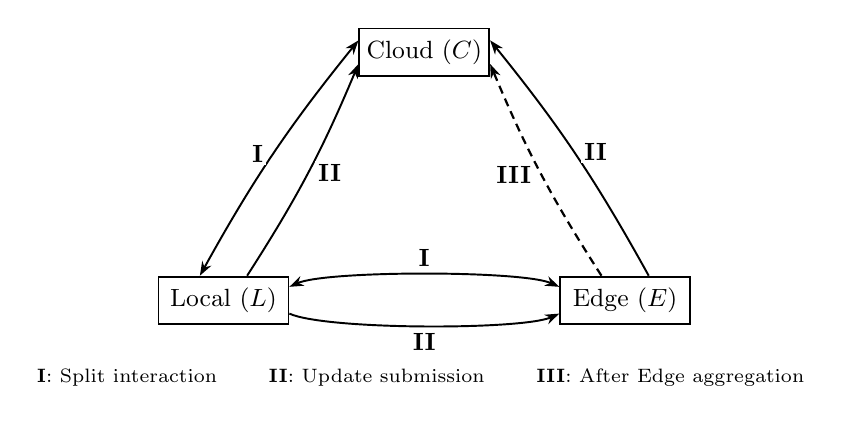
\begin{tikzpicture}[
        x=1cm,
        y=1cm,
        >={Stealth[length=1.8mm,width=1.3mm]},
        tier/.style={
            draw,
            rectangle,
            line width=0.65pt,
            minimum width=1.65cm,
            minimum height=0.60cm,
            inner sep=2pt,
            align=center,
            font=\small
        },
        pathI/.style={<->,line width=0.70pt},
        pathII/.style={->,line width=0.70pt},
        pathIII/.style={
            ->,
            dashed,
            dash pattern=on 3pt off 2pt,
            line width=0.80pt
        },
        ilab/.style={
            fill=white,
            inner sep=1pt,
            font=\small\bfseries
        }
    ]

    % Tiers
    \node[tier] (L) at (-2.55,0) {Local (\(L\))};
    \node[tier] (E) at ( 2.55,0) {Edge (\(E\))};
    \node[tier] (C) at ( 0,3.15) {Cloud (\(C\))};

    % ---------------------------------------------------------
    % Local -- Edge
    % ---------------------------------------------------------
    \draw[pathI]
        ([yshift=1.7mm]L.east)
        .. controls (-1.25,0.38) and (1.25,0.38) ..
        node[midway, above=0.5mm, ilab] {I}
        ([yshift=1.7mm]E.west);

    \draw[pathII]
        ([yshift=-1.7mm]L.east)
        .. controls (-1.25,-0.38) and (1.25,-0.38) ..
        node[midway, below=0.5mm, ilab] {II}
        ([yshift=-1.7mm]E.west);

    % ---------------------------------------------------------
    % Local -- Cloud
    % ---------------------------------------------------------
    \draw[pathI]
        ([xshift=-3.0mm]L.north)
        to[bend left=5]
        node[pos=0.50, left=0.8mm, ilab] {I}
        ([yshift=1.5mm]C.west);

    \draw[pathII]
        ([xshift=3.0mm]L.north)
        to[bend right=5]
        node[pos=0.50, right=0.8mm, ilab] {II}
        ([yshift=-1.5mm]C.west);

    % ---------------------------------------------------------
    % Edge -- Cloud
    % ---------------------------------------------------------
    \draw[pathII]
        ([xshift=3.0mm]E.north)
        to[bend right=5]
        node[pos=0.51, right=0.8mm, ilab] {II}
        ([yshift=1.5mm]C.east);

    \draw[pathIII]
        ([xshift=-3.0mm]E.north)
        to[bend left=5]
        node[pos=0.49, left=0.8mm, ilab] {III}
        ([yshift=-1.5mm]C.east);

    % ---------------------------------------------------------
    % Interface meanings
    % ---------------------------------------------------------
    \node[
        align=left,
        font=\scriptsize,
        anchor=north
    ] at (0,-0.75) {
        \textbf{I}: Split interaction
        \qquad
        \textbf{II}: Update submission
        \qquad
        \textbf{III}: After Edge aggregation
    };

    \end{tikzpicture}

    \vspace{-0.15cm}
    \caption{Collaboration interfaces and their physical positions in the
    cloud-edge-end architecture.}
    \label{fig:collaboration_graph}
\end{figure}
Based on these interfaces, we consider seven
client-level collaboration modes:
\begin{equation}
\mathcal H=
\{\mathrm{LIE},\mathrm{LIIE},\mathrm{LIC},\mathrm{LIIC},
\mathrm{LIEIIC},\mathrm{LIEIIIC},\mathrm{LIIEIIIC}\}.
\label{eq:seven_modes}
\end{equation}
For instance, LIE (\(L\)-I-\(E\)) enables split
training between the Local and Edge tiers,
whereas LIEIIC additionally forwards the resulting
update from the Edge to the Cloud through
Interface II. In LIEIIIC
(\(L\)-I-\(E\)-III-\(C\)), split training and
Edge aggregation are repeated before the
aggregated Edge update is transmitted to the
Cloud through Interface III.

Under split training modes, the model is partitioned
across the participating tiers, with
\(M_L^{h_i^t}\), \(M_E^{h_i^t}\), and
\(M_C^{h_i^t}\) denoting the model components
assigned to the Local, Edge, and Cloud tiers,
respectively. In contrast, local training modes
perform model training on the client before
transmitting the resulting update for aggregation.
In all seven modes, raw training data remain
on the client.

\subsubsection{Collaborative Link Blocks and Mode Flows}
We characterize each collaboration mode using
two basic training blocks. The split training
block \(S_{Lr}(L_B)\), where \(r\in\{E,C\}\),
represents \(L_B\) training steps performed
jointly by the Local tier and the Edge or
Cloud tier through split learning. The local
training block \(T_L(L_B)\) represents
\(L_B\) training steps performed entirely
at the Local tier, followed by the generation
of a model update for aggregation. Here,
\(L_B\) denotes the number of training steps
in each block.

The collaboration flow of each mode specifies
the sequence of training, update transmission,
and aggregation. Let \(A_E\) and \(A_C\)
denote Edge and Cloud aggregation, respectively.
For hierarchical modes, \(E_B\) denotes the
number of Edge-level training and aggregation
stages performed before the aggregated update
is forwarded to the Cloud.

With these definitions, the seven mode flows are
\begin{equation}
\begin{aligned}
\mathrm{LIE}:~~&
S_{LE}(L_B) \rightarrow A_E,\\
\mathrm{LIIE}:~~&
T_L(L_B) \xrightarrow{L\to E:\mathrm{upd}} A_E,\\
\mathrm{LIC}:~~&
S_{LC}(L_B) \rightarrow A_C,\\
\mathrm{LIIC}:~~&
T_L(L_B) \xrightarrow{L\to C:\mathrm{upd}} A_C,\\
\mathrm{LIEIIC}:~~&
S_{LE}(L_B)
\xrightarrow{E\to C:\mathrm{upd}} A_C,\\
\mathrm{LIEIIIC}:~~&
\bigl[S_{LE}(L_B)\rightarrow A_E\bigr]^{E_B}
\xrightarrow{E\to C:\mathrm{upd}} A_C,\\
\mathrm{LIIEIIIC}:~~&
\bigl[
T_L(L_B)
\xrightarrow{L\to E:\mathrm{upd}} A_E
\bigr]^{E_B}
\xrightarrow{E\to C:\mathrm{upd}} A_C .
\end{aligned}
\label{eq:mode_flows}
\end{equation}
Here, labeled arrows indicate model-update
transmissions between tiers, while unlabeled
arrows indicate the progression between training
and aggregation stages.

Figure~\ref{fig:eecblockflow} illustrates
the training and aggregation processes of
the seven collaboration modes.
Orange lines represent training blocks,
each consisting of \(L_B\) training steps.
Green lines indicate repeated training and
aggregation stages at the Edge in LIEIIIC
and LIIEIIIC, where \(E_B\) denotes the
number of repetitions.
Black loops represent aggregation operations,
while black arrows indicate the transmission
of model updates and the return of model
parameters among the Local, Edge, and Cloud.
These processes are used to define the
transmission set \(\mathcal X_i^t(h)\)
introduced below.

\begin{figure*}[t]
\centering
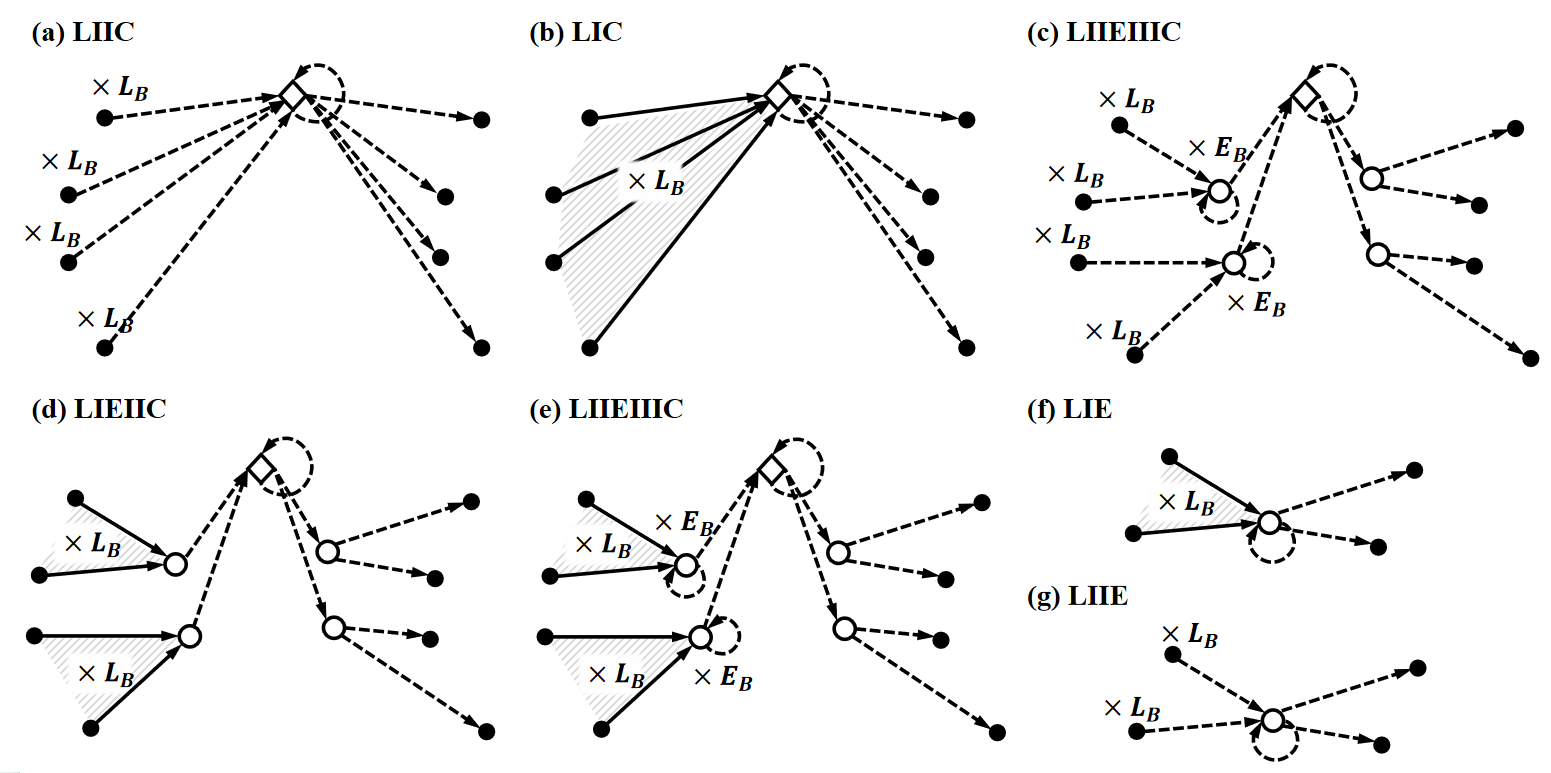
\includegraphics[width=\textwidth]{eecblockflow.png}
\caption{Execution structures of the seven collaboration modes in the cloud-edge-end architecture.}
\label{fig:eecblockflow}
\end{figure*}

\subsubsection{Mode Induced Transmission and Protection}
\begin{definition}[Transmission set induced by a mode]
For device \(i\), round \(t\), and collaboration
mode \(h\), define
\begin{equation}
\mathcal X_i^t(h)
=
\left\{
(u,v,b,n)
\;\middle|\;
(u,v,b)\text{ occurs }n\text{ times under }h
\right\}.
\label{eq:transmission_set}
\end{equation}
Here \(u,v\in\{L,E,C\}\), \(b\in\mathcal B\),
and \(n\) is the multiplicity of the directed
transmission in one complete mode flow.
The set of transmitted information is defined as
\begin{equation*}
\mathcal B=
\{\mathrm{emb},\mathrm{logits},\mathrm{grad},
\mathrm{emb\_grad},\mathrm{upd}\}.
\end{equation*}
Here, \(\mathrm{emb}\) denotes the intermediate
representation generated by the local model,
and \(\mathrm{logits}\) denotes the predictions
returned by the remote model.
The terms \(\mathrm{grad}\) and
\(\mathrm{emb\_grad}\) represent the gradients
with respect to the predictions and the
transmitted representations, respectively.
Finally, \(\mathrm{upd}\) denotes a model
update transmitted for aggregation or
model synchronization.
Together, these information types characterize
the transmissions associated with each
collaboration mode.
\end{definition}
For each transmission in \(\mathcal X_i^t(h)\),
the protection scheme is represented by
\[
\pi_i^{t,h}(u,v,b)
\in
\{\mathrm{none},\mathrm{HE},\mathrm{DP},
\mathrm{HE{+}DP}\},
\]
where the four values represent no protection,
homomorphic encryption, differential privacy,
and their combination, respectively.
The protection scheme for each transmission
is determined by its privacy requirements.

\subsection{Lifetime Privacy Accounting}
\label{sec:privacy_model}

We consider differential privacy protection
for model updates transmitted during training.
For client \(i\) in round \(t\), the update
transmissions requiring DP protection under
mode \(h\) are given by
\begin{equation}
\begin{aligned}
\mathcal D_i^t(h)
=
\bigl\{
&(u,v,b,n)\in\mathcal X_i^t(h)
\;\bigm|\;
b=\mathrm{upd},\\
&\pi_i^{t,h}(u,v,b)
\in\{\mathrm{DP},\mathrm{HE{+}DP}\}
\bigr\}.
\end{aligned}
\label{eq:dp_exposures}
\end{equation}
The set \(\mathcal D_i^t(h)\) identifies
the update transmissions requiring DP protection,
whereas privacy loss is accumulated only for
the corresponding DP releases that are
actually performed with calibrated Gaussian noise.

For each client, we use R\'enyi differential
privacy (RDP)~\cite{mironov2017renyi} to
accumulate privacy loss across training rounds.
Let \(\mathcal A\) denote the set of R\'enyi
orders.
For each release, Gaussian noise is calibrated
to the sensitivity of the model update.
Given a noise multiplier \(\sigma\), the
RDP cost at order \(\alpha\in\mathcal A\) is
\begin{equation}
\rho(\alpha,\sigma)
=
\frac{\alpha}{2\sigma^2}.
\label{eq:rdp_event_cost}
\end{equation}

Let \(m_i^t\) denote the number of Gaussian DP
releases actually performed for client \(i\)
in round \(t\), with corresponding noise
multipliers
\(\sigma_{i,1}^t,\ldots,\sigma_{i,m_i^t}^t\).
The accumulated RDP cost is updated as
\begin{equation}
\Phi_i^{t+1}(\alpha)
=
\Phi_i^t(\alpha)
+
\sum_{k=1}^{m_i^t}
\rho(\alpha,\sigma_{i,k}^t).
\label{eq:rdp_update}
\end{equation}
For a given \(\delta\), the accumulated RDP state is converted to the
corresponding privacy loss as
\begin{equation}
\epsilon_i^t
=
\min_{\alpha\in\mathcal A}
\left[
\Phi_i^t(\alpha)
+
\frac{\log(1/\delta)}{\alpha-1}
\right].
\label{eq:rdp_to_dp}
\end{equation}
The accumulated privacy loss of each client
must satisfy \(\epsilon_i^t\le\bar{\epsilon}\)
throughout training.

The noise multiplier depends on the number
of DP releases considered over the remaining
training rounds. For candidate mode \(h\),
this number is given by
\begin{equation}
N_i^t(h)
=
(R-t+1)
\sum_{(u,v,b,n)\in\mathcal D_i^t(h)}n,
\label{eq:planned_update_events}
\end{equation}
where \(R-t+1\) includes the current round.

For a candidate mode \(h\) with \(N_i^t(h)>0\),
the noise multiplier \(\sigma_i^t(h)\) is
numerically determined from the current RDP
state \(\{\Phi_i^t(\alpha)\}_{\alpha\in\mathcal A}\),
the release count \(N_i^t(h)\), and the
privacy target \((\bar{\epsilon},\delta)\).
The selected multiplier must keep the
projected privacy loss within
\(\bar{\epsilon}\), as evaluated using
\eqref{eq:rdp_to_dp}.
If no feasible noise multiplier is found,
the candidate mode is excluded.
When \(N_i^t(h)=0\), no noise calibration
is required.

For a hierarchical Edge group \(g\), the Edge update is released to the Cloud as a single packet with DP protection. The noise
multiplier used for this packet is derived from the calibrated client
multipliers of the participating devices as
\begin{equation}
\sigma_g^t
=
\max_{i\in\mathcal G_g}
\sigma_i^t(h_i^t).
\label{eq:edge_group_noise_multiplier}
\end{equation}
After a mode is selected and executed, only the DP events generated in
that round are added to \(\Phi_i^t(\alpha)\) according to
\eqref{eq:rdp_update}. The updated privacy state is then used to evaluate
the candidate modes in the next round.
\subsection{Joint Cost and Utility Modeling}
\label{sec:cost_utility_model}
Given the link topology, each mode induces its transmissions and the corresponding protection. Its privacy feasibility is determined by the lifetime accounting in Sec.~\ref{sec:privacy_model}. Each mode is then evaluated by resource feasibility, path latency, and learning error objective.
\subsubsection{End Side Resource Feasibility}
\label{sec:end_resource}

Each collaboration mode must satisfy the computation and memory capacities
of the end device. Let \(W_{i,L}^{\mathrm{comp}}(h_i)\) and
\(M_{i,L}^{\mathrm{mem}}(h_i)\) denote the profiled computation and memory
requirements of device \(i\) under mode \(h_i\), and let
\(Q_{\mathrm{comp},i}\) and \(Q_{\mathrm{mem},i}\) denote the corresponding
available capacities. The resource feasible mode set is

\begin{equation}
\mathcal H_i^{\mathrm{res}}
=
\left\{
h_i\in\mathcal H
\mid
W_{i,L}^{\mathrm{comp}}(h_i)\le Q_{\mathrm{comp},i},
\;
M_{i,L}^{\mathrm{mem}}(h_i)\le Q_{\mathrm{mem},i}
\right\}.
\label{eq:resource_feasible}
\end{equation}

If at least one full local update mode belongs to
\(\mathcal H_i^{\mathrm{res}}\), the candidate set
is restricted to the resource feasible full local
update modes. Otherwise, split interaction modes
are considered. A mode requiring DP protection is retained only
if a feasible noise multiplier can be determined
from the privacy target \((\bar\epsilon,\delta)\),
the current RDP state \(\Phi_i^t(\alpha)\),
and the release count \(N_i^t(h_i)\).
\subsubsection{Path and Round Latency on a Common Timeline}
We place the execution, transmission, and
aggregation events of the selected collaboration
modes on a common timeline to determine their
arrival times and the resulting round latency.

\textbf{Transmission latency.}
For a payload \(b\) transmitted from tier \(u\)
to tier \(v\), let \(S_{u,v,b}^t(h_i)\) denote
its original size, \(B_{i,u,v}^t\) the link
transmission rate for client \(i\), and
\(D_{u,v}^{0}\) the fixed link delay.
Under protection scheme
\(\pi_i^{t,h_i}(u,v,b)\), the transmission
latency is
\begin{equation}
T_{u,v,b}^{\mathrm{link},t}(h_i)
=
\frac{
\kappa\!\left(\pi_i^{t,h_i}(u,v,b)\right)
S_{u,v,b}^t(h_i)}
{B_{i,u,v}^t}
+
D_{u,v}^{0}
+
T_{u,v,b}^{\mathrm{priv},t}
\!\left(\pi_i^{t,h_i}(u,v,b)\right).
\label{eq:comm_latency}
\end{equation}
Here, \(\kappa(\cdot)\) denotes the payload
expansion factor, and
\(T_{u,v,b}^{\mathrm{priv},t}(\cdot)\)
denotes the protection processing time.
For unprotected transmissions,
\(\kappa(\mathrm{none})=1\) and
\(T_{u,v,b}^{\mathrm{priv},t}(\mathrm{none})=0\).

\textbf{Execution latency.}
Let \(\tau_{i,L}^t(h_i)\) and
\(\tau_{i,E}^t(h_i)\) denote the estimated
execution times per training step at the
Local and Edge tiers, respectively.
For Local--Edge split modes, the latency
model assumes pipelined execution across
\(L_B\) training steps, giving
\begin{equation}
T_i^{\mathrm{stage},t}(h_i)
=
L_B\max\!\left\{
\tau_{i,L}^t(h_i),\tau_{i,E}^t(h_i)
\right\}
+
\min\!\left\{
\tau_{i,L}^t(h_i),\tau_{i,E}^t(h_i)
\right\}.
\label{eq:execution_latency}
\end{equation}
For full local training,
\(T_i^{\mathrm{stage},t}(h_i)
=L_B\tau_{i,L}^t(h_i)\).
For modes with repeated training stages,
the corresponding stage duration is
multiplied by \(E_B\).

\textbf{Reconfiguration latency.}
Changing the collaboration mode may require
redistributing model components across the
Local, Edge, and Cloud tiers.
We model the resulting reconfiguration delay as
\begin{equation}
T_i^{\mathrm{sw},t}
=
\eta_h \mathbb{I}(h_i^t\neq h_i^{t-1})
+
\eta_p
\frac{
\|\mathbf{p}(h_i^t)-\mathbf{p}(h_i^{t-1})\|_1
}{2},
\label{eq:switching_cost}
\end{equation}
where \(\eta_h\) and \(\eta_p\) are the coefficients for the mode change cost and the placement change cost, respectively~\cite{CHEN2026112204,li2026latency}. The normalized model placement is
\begin{equation}
\mathbf{p}(h)
=
\frac{
\left[
\lvert M_L^{h}\rvert,
\lvert M_E^{h}\rvert,
\lvert M_C^{h}\rvert
\right]
}{
\lvert M_L^{h}\rvert+
\lvert M_E^{h}\rvert+
\lvert M_C^{h}\rvert
}.
\label{eq:model_placement_vector}
\end{equation}

\textbf{Path arrival and aggregation.}
For each candidate mode \(h_i\), the mode flow
determines the sequence of execution stages
and payload transmissions leading to the
relevant aggregation point.
We calculate update arrival times by
following this sequence and accounting for
execution, transmission, and reconfiguration
delays in their order of occurrence.
Let \(a_{i,E}^t\) and \(a_{i,C}^t\) denote
the arrival times of client \(i\)'s update
at the Edge and Cloud, respectively,
when the corresponding aggregation point
is involved in the selected mode.

Given a selected mode profile
\(\mathbf h^t=(h_1^t,\ldots,h_N^t)\),
we place the resulting update arrivals
on the common timeline.
For an Edge aggregation group \(g\),
let \(\mathcal G_g\) denote its
participating clients.
Edge aggregation begins after all required
client updates have arrived.
Its completion time is
\begin{equation}
f_{g,E}^t
=
\max_{i\in\mathcal G_g} a_{i,E}^t
+
T_{g,E}^{\mathrm{agg},t},
\label{eq:edge_agg_finish}
\end{equation}
where \(T_{g,E}^{\mathrm{agg},t}\) is the Edge aggregation duration. Updates arriving earlier remain buffered until aggregation starts.

For modes that forward an Edge aggregation
result to the Cloud, transmission begins
after the Edge aggregation completes at
time \(f_{g,E}^t\).
Let \(a_{g,C}^t\) denote the arrival time
of this result at the Cloud, including
the Edge to Cloud transmission latency.
Modes that transmit updates directly
to the Cloud instead produce client
arrival times \(a_{i,C}^t\).
Cloud aggregation waits for all required
updates from the applicable paths.
Its completion time is
\begin{equation}
f_C^t
=
\max\left\{
\max_i a_{i,C}^t,\,
\max_g a_{g,C}^t
\right\}
+
T_C^{\mathrm{agg},t},
\label{eq:cloud_agg_finish}
\end{equation}
where the two maxima are taken over the direct Cloud clients and the Edge
groups participating in the current Cloud aggregation, respectively.

When required by a selected mode, return
transmissions are scheduled after the
corresponding aggregation completes.
As illustrated in Fig.~\ref{fig:time},
all execution, transmission, aggregation,
and return events are placed on a common
timeline according to their dependencies.
The system round latency
\(T_{\mathrm{sys}}(\mathbf h^t)\)
is the latest completion time among
all required events.
\begin{figure*}[t]
\centering
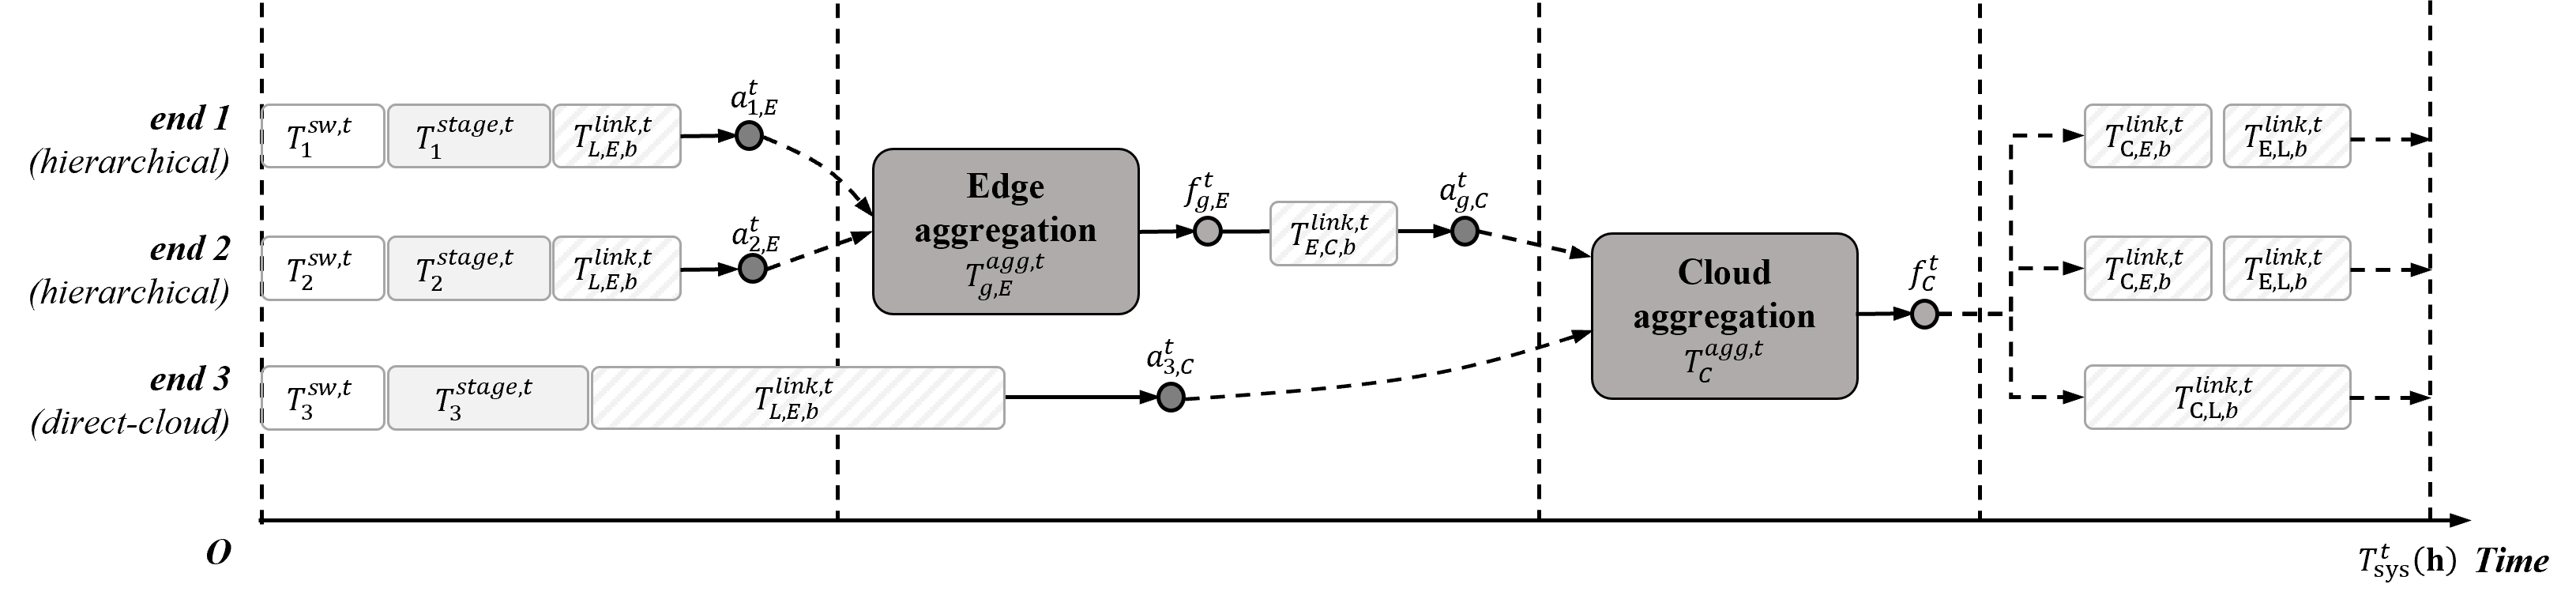
\includegraphics[width=\textwidth]{common_timeline.png}
\caption{Illustrative common timeline for
mixed collaboration modes, showing
hierarchical Edge aggregation and direct
Cloud updates. The system round latency
is determined by the latest completion
time of the required events.}
\label{fig:time}
\end{figure*}
\subsubsection{Learning Error and DP Perturbation Cost}
\label{sec:learning_cost}

The selector estimates the learning error of
each candidate mode profile using information
available at selection time.
We account for two sources of update error:
(i) fusion deviation due to incomplete
Cloud participation, and
(ii) stochastic noise introduced by
DP-protected update releases.

Differential privacy is accounted for at
actual protected release events.
We consider sample-level replacement adjacency,
where neighboring datasets differ in one
training sample of the same client.
Let \(C_u\) denote the clipping norm of a
released client update.
If the complete update is clipped to this norm,
its sensitivity is bounded by
\(\Delta_u=2C_u\).

For an update vector of dimension \(d_{\mathrm{upd}}\), a Gaussian mechanism
with noise multiplier \(\sigma\) and sensitivity \(\Delta\) introduces a
zero-mean perturbation whose expected squared norm is

\begin{equation}
\mathbb{E}
\left[
\left\|
z_{\mathrm{DP}}
\right\|_2^2
\right]
=
d_{\mathrm{upd}}
\left(
\sigma \Delta
\right)^2 .
\label{eq:gaussian_update_perturbation}
\end{equation}

For a client update released directly to the Cloud, the clipped client update
is perturbed before release, and its sensitivity is therefore
\(\Delta_u=2C_u\).

For hierarchical aggregation, the participating client updates are first
clipped and aggregated before the aggregate is released. Consider an Edge
group \(g\) with participating client set \(\mathcal G_g\). The aggregation
weight of client \(i\) within this group is

\begin{equation}
w_{i\mid g}
=
\frac{n_i}
{\sum_{j\in\mathcal G_g} n_j}.
\label{eq:edge_group_weight}
\end{equation}
Under sample-level replacement adjacency,
only one client's update can change.
With fixed aggregation weights and the
clipping bound defined above, the
sensitivity of the Edge aggregate is
bounded by
\begin{equation}
\Delta_g^t
=
2C_u
\max_{i\in\mathcal G_g}
w_{i\mid g}.
\label{eq:edge_group_sensitivity}
\end{equation}
An Edge aggregate contributes a DP release
to \(\mathcal R_{\mathrm{DP}}^t(\mathbf h^t)\)
only when calibrated Gaussian noise is
actually applied before its release to
the Cloud.
For this release, the noise multiplier is
\(\sigma_g^t\), as defined in
\eqref{eq:edge_group_noise_multiplier}.
Noise is added once to the aggregate,
rather than separately to its constituent
client updates at this release boundary.

The same release-boundary principle applies to other aggregate releases. When
multiple clipped client updates are securely aggregated before a DP-protected
release, the released aggregate is treated as one DP release object, and its
sensitivity is determined by the largest normalized client contribution in
that aggregate.

For a complete collaboration profile
\(\mathbf h^t=(h_1^t,\ldots,h_N^t)\), let
\(\mathcal R_{\mathrm{DP}}^t(\mathbf h^t)\) denote the set of effective
DP-protected update releases that contribute to the current Cloud update.
Each release \(q\in\mathcal R_{\mathrm{DP}}^t(\mathbf h^t)\) may correspond
to either an individually released client update or an aggregate update.
Let \(\omega_q^t\) denote the weight of release \(q\) in the resulting Cloud
aggregation, let \(\sigma_q^t\) denote its noise multiplier, and let
\(\Delta_q^t\) denote its sensitivity at the corresponding release boundary.
The DP perturbation cost of profile \(\mathbf h^t\) is then

\begin{equation}
J_{\mathrm{DP}}(\mathbf h^t)
=
d_{\mathrm{upd}}
\sum_{q\in\mathcal R_{\mathrm{DP}}^t(\mathbf h^t)}
\left(
\omega_q^t
\sigma_q^t
\Delta_q^t
\right)^2 .
\label{eq:dp_perturbation_cost}
\end{equation}

For a directly released client update \(i\), the release sensitivity is
\(\Delta_q^t=\Delta_u\), and its Cloud aggregation weight is determined by
the represented sample mass. For an Edge aggregate release from group \(g\),
the release sensitivity is \(\Delta_q^t=\Delta_g^t\), and its Cloud
aggregation weight is determined by the total sample mass represented by that
Edge group. Therefore, \eqref{eq:dp_perturbation_cost} evaluates DP
perturbation according to the actual released object rather than according to
the number of client updates contained in that object.

In addition to DP perturbation, collaboration modes that terminate at the Edge
without forwarding their updates to the Cloud omit part of the training sample
mass from the current global aggregation. Let

\begin{equation}
N_{\mathrm{total}}
=
\sum_{i=1}^{N} n_i
\label{eq:total_sample_mass}
\end{equation}

denote the total training sample mass across all clients. Let
\(N_C^t(\mathbf h^t)\) denote the sample mass represented in the current Cloud
aggregation. The corresponding Cloud coverage ratio is

\begin{equation}
r_C^t(\mathbf h^t)
=
\frac{
N_C^t(\mathbf h^t)
}{
N_{\mathrm{total}}
}.
\label{eq:cloud_mass_ratio}
\end{equation}

When \(r_C^t(\mathbf h^t)<1\), the update produced by the selected
collaboration profile deviates from the full-participation federated update.
As shown in Proposition~\ref{prop:learning_bound}, the squared norm of this
fusion deviation is bounded by

\begin{equation}
J_{\mathrm{fusion}}^t(\mathbf h^t)
=
4C_u^2
\left(
1-r_C^t(\mathbf h^t)
\right)^2 .
\label{eq:fusion_cost}
\end{equation}

Under a \(\beta\)-smooth global loss and step size
\(\eta\le 1/\beta\), Proposition~\ref{prop:learning_bound} further shows that
the profile-dependent part of the one-round expected loss increment is bounded
by the fusion deviation and the DP perturbation variance with a common
positive scaling factor. Since this common factor does not affect the ordering
of candidate profiles, the selection-time learning objective is defined as

\begin{equation}
\widehat J_{\mathrm{learn}}^t(\mathbf h^t)
=
4C_u^2
\left(
1-r_C^t(\mathbf h^t)
\right)^2
+
J_{\mathrm{DP}}(\mathbf h^t).
\label{eq:j_learn_objective}
\end{equation}

For an Edge-only profile with
\(r_C^t(\mathbf h^t)=0\), no DP-protected update is released to the Cloud.
We therefore define

\begin{equation}
J_{\mathrm{DP}}(\mathbf h^t)=0
\qquad
\text{when}
\qquad
r_C^t(\mathbf h^t)=0 .
\label{eq:edge_only_dp_cost}
\end{equation}

In this case, the learning objective reduces to

\begin{equation}
\widehat J_{\mathrm{learn}}^t(\mathbf h^t)
=
4C_u^2 ,
\end{equation}

which is the maximum value of the fusion-deviation bound. Hence, a profile
that completely abandons Cloud fusion is not evaluated as a zero-cost
solution.

\subsection{Global Multiobjective Collaborative Optimization}
\label{sec:global_optimization}

For each client, the decision variable is the collaboration mode
\(h_i^t\in\mathcal F_i^t\), where
\(\mathcal F_i^t\subseteq\mathcal H_i^{\mathrm{res}}\subseteq\mathcal H\)
contains the modes that satisfy the end device resource constraints in
\eqref{eq:resource_feasible}, the mechanism requirements of each exposure,
and the lifetime privacy constraint. For each evaluated mode, \(\mathcal X_i^t(h_i)\) is induced first. The exposure requirements then determine the protection map \(\pi_i^{t,h_i}\), and the current privacy ledger determines the noise multiplier \(\sigma_{i,h_i}^t\) when a protected update needs DP. Thus \(\pi_i^{t,h_i}\) and \(\sigma_{i,h_i}^t\) follow from the candidate mode.

A complete mixed mode profile is \(\mathbf h^t=(h_1^t,\ldots,h_N^t)\). The flow evaluator applies the shared Edge and Cloud aggregation and admission rules to a complete profile, so the system feasible set is a subset of the Cartesian product,
\begin{equation}
\mathcal F_{\mathrm{sys}}^t
\subseteq
\prod_{i=1}^{N}\mathcal F_i^t.
\label{eq:global_feasible_set}
\end{equation}
An execution that is not admitted is reported as \textsc{skip}.

For every feasible profile, the flow model produces the round duration $T_{\mathrm{sys}}(\mathbf h^t)$, while the formal learning objective $\widehat J_{\mathrm{learn}}^t(\mathbf h^t)$ is evaluated through \eqref{eq:j_learn_objective}. The selector therefore minimizes the following two objective functions:
\begin{equation}
\underset{\mathbf h^t\in\mathcal F_{\mathrm{sys}}^t}
{\operatorname{minimize}}
\quad
\mathbf f(\mathbf h^t)
=
\begin{bmatrix}
T_{\mathrm{sys}}(\mathbf h^t)\\
\widehat J_{\mathrm{learn}}^t(\mathbf h^t)
\end{bmatrix}.
\label{eq:global_multiobjective}
\end{equation}

Latency and the learning error are the two objectives in the current implementation. HE and communication processing contribute to the path latency, while partial Cloud participation and DP calibration jointly determine the expected learning error bound.

The nondominated decision set is
\begin{equation}
\mathcal H_{\mathrm P}^t
=
\left\{
\mathbf h^t\in\mathcal F_{\mathrm{sys}}^t
\;\middle|\;
\nexists\,\mathbf h^{\prime t}\in\mathcal F_{\mathrm{sys}}^t
\text{ such that }
\mathbf h^{\prime t}\prec\mathbf h^t
\right\},
\label{eq:pareto_front}
\end{equation}
where \(\prec\) denotes Pareto dominance with respect to the two objectives in \eqref{eq:global_multiobjective}. In the bounded solver, the maintained nondominated archive approximates this set.

The Tchebycheff stage normalizes the two objectives over the current nondominated archive. Let $T_{\min}^t,T_{\max}^t$ and $J_{\min}^t,J_{\max}^t$ denote the minimum and maximum values of the latency and learning error objectives observed in that archive. These values define the normalization range within the current archive. The normalized objectives are
\begin{equation}
\bar T(\mathbf h^t)
=
\frac{
T_{\mathrm{sys}}(\mathbf h^t)-T_{\min}^t
}{
T_{\max}^t-T_{\min}^t+\gamma_n
},
\qquad
\bar J(\mathbf h^t)
=
\frac{
\widehat J_{\mathrm{learn}}^t(\mathbf h^t)-J_{\min}^t
}{
J_{\max}^t-J_{\min}^t+\gamma_n
}.
\label{eq:pareto_normalization}
\end{equation}

The normalized ideal point is the origin. The selected profile minimizes the largest normalized deviation,
\begin{equation}
\begin{aligned}
D_\infty(\mathbf h^t)
&=
\max\left\{
\left|\bar T(\mathbf h^t)\right|,
\left|\bar J(\mathbf h^t)\right|
\right\},
\\
\mathbf h^{t\star}
&\in
\arg\min_{\mathbf h^t\in\mathcal H_{\mathrm P}^t}
D_\infty(\mathbf h^t).
\end{aligned}
\label{eq:selection}
\end{equation}

The implementation resolves equal distances deterministically using system latency, then \(\widehat J_{\mathrm{learn}}^t(\mathbf h^t)\), followed by a stable profile identity. Real test accuracy is reserved for experimental evaluation.
\section{Algorithm}
\label{sec:algorithm}

The proposed selection procedure operates at strategy update points. At
rounds that are not update points, the previously selected profile is reused
when \(\mathbf h^{t-1}\in\mathcal F_{\mathrm{sys}}^t\).

\begin{breakablealgorithm}
\caption{Bounded Pareto Profile Selection with Exposure Specific Protection}
\label{alg:selection}
\small
\begin{algorithmic}[1]

\REQUIRE
\(N,\{\mathcal H_i^{\mathrm{res}}\}_{i=1}^{N},
\{\Phi_i^t(\alpha)\}_{i=1}^{N},
(\bar\epsilon,\delta)\), system state, \(S_P\),
\(K_{\mathrm P},K_{\mathrm B},I_{\max},\mathbf h^{t-1}\)

\ENSURE
\(\mathbf h^{t\star}\), or \textsc{skip}

\STATE \textbf{Reuse}

\IF{\(t\notin S_P\) and \(\mathbf h^{t-1}\in\mathcal F_{\mathrm{sys}}^t\)}
    \STATE Execute \(\mathbf h^{t-1}\) with its protection mechanisms
    \STATE Update \(\Phi_i^{t+1}(\alpha)\) using \eqref{eq:rdp_update} for
    executed and released DP events only
    \RETURN \(\mathbf h^{t-1}\)
\ENDIF

\STATE \textbf{Candidate Construction}

\FOR{\(i=1,\ldots,N\)}
    \STATE \(\mathcal F_i^t\leftarrow\emptyset\)
    \STATE Apply resource-aware split activation: if
    \(\mathcal H_i^{\mathrm{res}}\) contains at least one full-local
    update mode, retain only the full-local modes; otherwise also
    admit the split-interaction modes
    \FOR{each activated \(h_i\in\mathcal H_i^{\mathrm{res}}\)}
        \STATE Construct \(\mathcal X_i^t(h_i)\) and derive
        \(\pi_i^{t,h_i}\), \(\mathcal D_i^t(h_i)\) by
        \eqref{eq:transmission_set}--\eqref{eq:dp_exposures}
        \STATE Compute \(N_i^t(h_i)\) by
        \eqref{eq:planned_update_events}
        \IF{\(N_i^t(h_i)>0\)}
            \STATE Calibrate \(\sigma_i^t(h_i)\) under
            \((\bar\epsilon,\delta)\)
            \IF{no feasible \(\sigma_i^t(h_i)\) exists}
                \STATE \textbf{continue}
            \ENDIF
        \ENDIF
        \STATE Add \(h_i\) to \(\mathcal F_i^t\)
    \ENDFOR
\ENDFOR

\STATE \textbf{Pareto Search}

\STATE Construct
\(\mathcal F_{\mathrm{sys}}^t\subseteq\prod_{i=1}^{N}\mathcal F_i^t\)
using the shared flow, buffer, aggregation, and admission constraints
\STATE Generate a bounded initial candidate set from
\(\mathcal F_{\mathrm{sys}}^t\)

\IF{\(\mathcal F_{\mathrm{sys}}^t=\emptyset\)}
    \RETURN \textsc{skip}
\ENDIF

\STATE Evaluate the initial candidate profiles using
\(T_{\mathrm{sys}}(\mathbf h^t)\) and \(\widehat J_{\mathrm{learn}}^t(\mathbf h^t)\) via \eqref{eq:j_learn_objective}

\STATE Initialize archive \(\mathcal A\) with the nondominated initial
profiles and queue \(\mathcal B\)

\FOR{\(r=1,\ldots,I_{\max}\)}
    \STATE Generate unvisited single client replacements from
    \(\mathcal A\cup\mathcal B\)
    \STATE Retain only profiles in \(\mathcal F_{\mathrm{sys}}^t\)
    \STATE Evaluate \(T_{\mathrm{sys}}(\mathbf h^t)\) and
    \(\widehat J_{\mathrm{learn}}^t(\mathbf h^t)\) via \eqref{eq:j_learn_objective} for the retained profiles
    \STATE Update \(\mathcal A\), keeping at most \(K_{\mathrm P}\)
    nondominated profiles
    \STATE Update \(\mathcal B\), keeping at most \(K_{\mathrm B}\)
    exploratory profiles
    \IF{neither \(\mathcal A\) nor \(\mathcal B\) is updated}
        \STATE \textbf{break}
    \ENDIF
\ENDFOR

\STATE Set \(\widehat{\mathcal H}_{\mathrm P}^t\leftarrow\mathcal A\)

\STATE \textbf{Profile Selection}

\STATE Normalize the two objectives over
\(\widehat{\mathcal H}_{\mathrm P}^t\) by
\eqref{eq:pareto_normalization}

\STATE Select
\[
\mathbf h^{t\star}\in
\arg\min_{\mathbf h^t\in\widehat{\mathcal H}_{\mathrm P}^t}
D_\infty(\mathbf h^t)
\]
with the specified deterministic tie breaking rule

\STATE \textbf{Execution and Accounting}

\STATE Execute \(\mathbf h^{t\star}\) and its protection mechanisms

\STATE Update \(\Phi_i^{t+1}(\alpha)\) using \eqref{eq:rdp_update} for
executed and released DP events only

\RETURN \(\mathbf h^{t\star}\)

\end{algorithmic}
\end{breakablealgorithm}
\section{Experiments}
\label{sec:experiment}
\subsection{Experimental Setup}
\label{sec:exp_setup}
The formal CIFAR 10 protocol uses real model training together with the system
simulator. Its current configuration, \texttt{paper\_flow\_v31\_mode\_specific\_privacy},
contains 100 end devices, 10 edge nodes, and one cloud node and schedules 100
communication rounds. The model is a pretrained ResNet 18 with only its
classification head trained. Each private training stage uses three local epochs
and a learning rate of 0.01. LIEIIIC and LIIEIIIC use three edge stages; the
other executable modes use one. The configured formal seeds are 40, 42, and 44.
The 100-round, three-seed configuration specifies the intended formal evaluation;
numerical tables remain pending until runs under this execution revision are
complete. Fashion MNIST with LeNet 5 is retained as a secondary evaluation target,
but legacy outputs produced under earlier execution revisions are not mixed with
the current formal results. The main parameters are listed in
\tabref{tab:sim_params}.

\begin{table*}[t]
\centering
\caption{Default Simulation Parameters}
\label{tab:sim_params}
\scriptsize
\setlength{\tabcolsep}{3pt}
\begin{tabularx}{\textwidth}{@{}>{\raggedright\arraybackslash}p{0.20\textwidth}>{\centering\arraybackslash}p{0.27\textwidth}>{\raggedright\arraybackslash}p{0.20\textwidth}>{\centering\arraybackslash}X@{}}
\hline
\textbf{Parameter} & \textbf{Value} & \textbf{Parameter} & \textbf{Value} \\
\hline
End and edge nodes & 100 end devices and 10 edge nodes & Training rounds & \(T=100\) \\
Training and test samples & 12000 and 2000 & Random seeds & 40, 42, and 44 \\
Client computation and memory factors & Independent $\mathcal U(0.5,2.0)$ & Edge computation factor & $\mathcal U(2/3,1.5)$ \\
Logical link block reference & \(L_B=5\) & Independent stages in multilevel modes & \(E_B=3\) \\
Lifetime update-DP target & \(\bar\epsilon=8.0\) & DP slack parameter & \(\delta=10^{-5}\) \\
Base transmission size & \(S_{\mathrm{emb}}=1.6\) MB, \(S_{\mathrm{upd}}=0.02052\) MB & HE expansion factor & \(\alpha_{\mathrm{HE}}=8.04\) \\
CKKS polynomial degree and scale & \(8192\) and \(2^{40}\) & CKKS coefficient modulus bits & \([50,40]\) \\
CKKS reference profile for a 4 MB update & 32.14 MB and 0.90 s & HE execution & Real SEAL when selected \\
Base link rates & end to edge 5, end to cloud 2.2, edge to cloud 8 MB/s & Rate variation & sinusoidal amplitude 0.2 and uniform jitter 0.25 \\
Aggregation fraction & $\rho_{\mathrm{buf}}=1.0$ & Strategy update period & $S_P=1$ \\
Update clip norm (CIFAR 10 head) & $C_u=0.25$ & Dynamic DP multiplier & Lifetime-aware $\sigma_{i,h}^t$ \\
Pareto archive, beam, and expansions & $K_{\mathrm P}=16$, $K_{\mathrm B}=4$, $I_{\max}=50$ & Cloud fusion penalty & $\xi=0.2$, $\varepsilon=0.05$ \\
Training hardware & Intel i7 11700F, GTX 1660 Ti 6 GB, 31.8 GB RAM & Software & Python 3.10.9, PyTorch 2.5.1, torchvision 0.20.1, SEAL 4.0.0 \\
\hline
\end{tabularx}
\end{table*}

The encrypted aggregator performs ciphertext addition without ciphertext
multiplication. The coefficient modulus therefore contains one 50 bit data
prime and one 40 bit special prime. Its total of 90 bits is below the 218 bit
limit reported by SEAL for polynomial degree 8192 at the 128 bit security
level.

The fixed link, switching, and aggregation profiles used by the analytical
latency model are listed in \tabref{tab:additional_profile_params}.
\begin{table}[t]
\centering
\caption{Additional Profiling Parameters}
\label{tab:additional_profile_params}
\small
\setlength{\tabcolsep}{4pt}
\begin{tabularx}{\columnwidth}{@{}lX@{}}
\hline
\textbf{Parameter} & \textbf{Value used in the experiments} \\
\hline
Base link delay \(D_{\lambda}^{0}\) & End to edge 0.015 s, end to cloud 0.040 s, and edge to cloud 0.010 s. Reverse links use the corresponding value. \\
Switching coefficients & \(\eta_h=0.02\) s and \(\eta_p=0.08\) s \\
Edge aggregation profile & \(\beta_j=0.01\) s/MB and \(T_j^{\mathrm{fix}}=0.02\) s \\
Cloud aggregation profile & \(\beta_C=0.015\) s/MB and \(T_C^{\mathrm{fix}}=0.04\) s \\
\hline
\end{tabularx}
\end{table}

The configured value \(S_{\mathrm{emb}}=1.6\) MB is the payload assigned to
one embedding transmission event in the analytical link model. The
corresponding backward gradient event uses the same payload profile. This value
is a reproducible simulation input rather than a per sample or per layer tensor
size.
The ResNet 18 update payload in the formal configuration contains the 5130
trainable classifier parameters stored as 32 bit floating point values, giving
20520 bytes before encryption. The CKKS processing profile uses 4 MB as its
reference granularity and scales linearly with the actual update payload.

The pretrained model uses \texttt{ResNet18\_Weights.DEFAULT} from torchvision.
The formal CIFAR 10 configuration is \texttt{resnet18\_pretrained\_head}:
only the 512-to-10 classifier weight and bias (5130 parameters) are trained.
The feature extractor and BatchNorm parameters and running statistics remain frozen.
Client-level clipping and Gaussian noise operate on the complete classifier update;
frozen backbone parameters are neither perturbed nor included in the encrypted update.
Thus the unencrypted float32 update contains 20520 bytes. This scope is distinct
from finetuning layer3 and layer4. The
split point is placed after \texttt{layer2}, as shown in
\tabref{tab:resnet_mode_mapping}. The same parameter partition is used by model
execution, transmitted update construction, and aggregation.

\begin{table*}[t]
\centering
\caption{ResNet 18 Execution and Aggregation Mapping}
\label{tab:resnet_mode_mapping}
\small
\setlength{\tabcolsep}{4pt}
\begin{tabularx}{\textwidth}{@{}lXXX@{}}
\hline
\textbf{Mode} & \textbf{End execution} & \textbf{Edge execution} & \textbf{Cloud role} \\
\hline
LIE & Frozen stem through layer2 & Downstream split execution and edge-side training & No Cloud update exposure \\
LIIE & Local classifier training & Receives and aggregates local updates & No Cloud update exposure \\
LIC & Frozen stem through layer2 & Relay only & Downstream split execution; no model-update upload \\
LIIC & Local classifier training & Not on the update path & Receives protected client update \\
LIEIIC & Frozen stem through layer2 & Downstream split execution and classifier training & Receives protected edge update \\
LIEIIIC & Frozen stem through layer2 & Three split/edge stages followed by edge aggregation & Receives protected edge update \\
LIIEIIIC & Three local/edge update stages & Aggregates staged local updates & Receives protected edge update \\
\hline
\end{tabularx}
\end{table*}

For each seed, a seeded permutation selects 12000 CIFAR 10 training samples
and 2000 test samples. Images use channel means
$(0.4914,0.4822,0.4465)$ and standard deviations
$(0.2023,0.1994,0.2010)$. Under the main moderate edge label skew, each label
is shared equally across two adjacent edge domains with cyclic wraparound, and
each edge therefore contains two neighboring labels. The samples assigned to
each edge are divided among its ten associated clients. The extreme edge label
skew variant used for stress testing instead assigns each label to one edge
domain. Each client then reserves 20\% of its assigned samples for validation.

Client computation and memory factors are independently drawn from
$\mathcal U(0.5,2.0)$, and edge computation factors are drawn from
$\mathcal U(2/3,1.5)$. Lower computation factors indicate faster execution.
For direction $u\rightarrow v$, the simulated rate in round $t$ is
\begin{equation}
R_{i,u,v}^{t}=\bar R_{u,v}[1+0.2\sin(t/3)]\zeta_{i,u,v}^{t},
\qquad \zeta_{i,u,v}^{t}\sim\mathcal U(0.75,1.25).
\label{eq:experiment_link_rate}
\end{equation}
The base rates are 5 MB/s for end to edge links, 2.2 MB/s for end to cloud
links, and 8 MB/s for edge to cloud links. Reverse links use the same base
rate. These values define a reproducible synthetic network scenario rather
than a physical network measurement.

Privacy execution follows the mode-specific exposure contract in
Section~\ref{sec:privacy_model}. A mode first determines its transmitted objects
and links. Under the current paper profile, a Cloud-facing model-update exposure
requires both client-level DP calibration and HE-protected aggregation, whereas
edge-only execution does not acquire an artificial Cloud release. For a dynamic
privacy candidate, the update multiplier is the minimum value feasible under the
client's current ledger and the protected update events planned over the remaining
training horizon. Consequently there is no single noise multiplier shared by all
modes and rounds. The CIFAR 10 classifier update is clipped at $C_u=0.25$ before
the applicable DP mechanism. When a selected candidate uses HE, the formal
configuration requires real SEAL execution; DP and HE retain their distinct
privacy-loss and confidentiality roles. Only DP events that are actually executed
and released are charged to the corresponding client ledger.

All four formal policies use the same data partition, optimizer, training work,
resource process, and flow model. The configured main-comparison seeds are 40,
42, and 44. Controlled studies should use the same seeds unless a study explicitly
states otherwise, and results from older execution revisions are not combined
with the current formal comparison.

Every run stores the complete configuration, runtime environment, exact client
partition, generated system profiles, model parameter partition, raw client
decisions, link events, and round metrics in its output directory.

The system time used for efficiency comparisons is the modeled cloud-edge-end
execution time plus the measured mode selection time. It includes the decision
cost while excluding the sequential host overhead caused by emulating many
clients on one machine. Host wall time is recorded separately as an
implementation measurement and is not used as deployment latency.

\subsection{CKKS Profile Validation}
\label{sec:ckks_validation}

The CKKS profile uses polynomial modulus degree 8192, coefficient modulus bits
\([50,40]\), scale \(2^{40}\), and chunks of at most 4096 values. A complete
historical one round ResNet 18 validation selected HE for 40 clients and encrypted 21.13 GB
of generated ciphertext. Encryption, ciphertext addition, and decryption took
335.78 s. The maximum absolute difference from plaintext aggregation was
\(9.17\times10^{-8}\). The profiled and encrypted executions produced the same
test accuracy, and their global update norms differed by
\(1.47\times10^{-9}\). These are historical full-model transport measurements, not validation results
for the current classifier-only, mode-specific privacy execution. The
5130-coordinate payload requires a fresh CKKS cost calibration; old costs must
not be presented as measured classifier-only system performance.
% The numerical tables and figures below must be regenerated with execution
% revision paper_flow_v31_mode_specific_privacy before submission.
\subsection{Compared Policies and Main Results}
The formal comparison isolates the two adaptive axes of DynFL: collaboration
mode and privacy calibration. \textsc{Fixed Mode + Fixed Privacy} restricts
executed clients to the fixed LIIEIIIC collaboration mode and reuses each
client's established protection profile. \textsc{Dynamic Mode + Fixed Privacy}
allows collaboration modes to adapt while holding that privacy profile fixed.
\textsc{Fixed Mode + Dynamic Privacy} keeps LIIEIIIC but recalibrates privacy
from the evolving ledger and remaining horizon. \textsc{Full DynFL} makes both
axes state dependent. Infeasible clients may produce \textsc{skip}; this is an
execution/admission outcome and not an additional collaboration mode.

All four policies are evaluated through the same candidate legality checks,
shared-resource flow model, system-level latency/error objectives, and actual
execution/accounting path. Thus ``fixed privacy'' does not mean that privacy is
disabled, and ``dynamic privacy'' does not introduce a separate privacy objective;
it changes the state-dependent calibration used by otherwise legal exposures.
The formal configuration also requires feasible execution, Edge/Cloud coverage,
and real HE whenever a selected candidate requires HE.

\tabref{tab:main_comparison} and \figref{fig:accuracy_convergence} are reserved
for the completed three-seed formal runs. The primary efficiency value is system
time, which combines modeled workflow execution with measured decision time. The
privacy column reports the realized update-level client privacy accounting under
the executed protected events. Results produced by earlier fused/global-release
execution revisions are not retained in this comparison because their privacy,
aggregation, feasible-set, and timing semantics differ from the current protocol.

\begin{table*}[t]
\centering
\caption{Main comparison on CIFAR 10 with ResNet 18 over 100 communication rounds. Values will report the mean and 95\% confidence interval over three random seeds}
\label{tab:main_comparison}
\scriptsize
\begin{adjustbox}{max width=\textwidth}
\begin{tabular}{lccccc}
\hline
\textbf{Method} & \textbf{Final Acc. (\%)} & \textbf{Last 10 Acc. (\%)} & \textbf{System Time (s)} & \textbf{Comm. (GB)} & \textbf{$\epsilon$} \\
\hline
Fixed Mode + Fixed Privacy & -- & -- & -- & -- & -- \\
Dynamic Mode + Fixed Privacy & -- & -- & -- & -- & -- \\
Fixed Mode + Dynamic Privacy & -- & -- & -- & -- & -- \\
Full DynFL & -- & -- & -- & -- & -- \\
\hline
\end{tabular}
\end{adjustbox}
\end{table*}
\FloatBarrier

\begin{figure}[t]
\centering
\IfFileExists{cifar10_resnet18_100r_wall_time_accuracy_v31.png}{
\includegraphics[width=\columnwidth]{cifar10_resnet18_100r_wall_time_accuracy_v31.png}
}{
\fbox{\parbox[c][4.5cm][c]{0.94\columnwidth}{\centering v31 main experiment figure pending}}
}
\caption{Raw test accuracy against system time on CIFAR 10 with ResNet 18. All curves use the common interval determined by the shortest completed run. The curves show the mean over three random seeds, the shaded regions show 95\% confidence intervals, and the inset enlarges the final quarter of the common interval.}
\label{fig:accuracy_convergence}
\end{figure}

\subsection{Reconfiguration Behavior}
\label{sec:reconfiguration_behavior}

The client decision logs expose how the selected workflow changes during
training. \figref{fig:reconfiguration_behavior} reports the share of clients in
each executable collaboration mode together with the realized protected-update
exposure coverage. The mode switch curve records the fraction of clients whose
selected mode differs from the preceding round. These measurements distinguish
dynamic workflow reconfiguration from a fixed topology with changing scalar
parameters.

\begin{figure}[t]
\centering
\IfFileExists{cifar10_reconfiguration_trace_v31.png}{
\includegraphics[width=\columnwidth]{cifar10_reconfiguration_trace_v31.png}
}{
\fbox{\parbox[c][4.5cm][c]{0.94\columnwidth}{\centering v31 reconfiguration figure pending}}
}
\caption{Raw collaboration mode shares, realized protected-update exposure coverage, and client mode switch rate over communication rounds. The curves report the mean over three random seeds.}
\label{fig:reconfiguration_behavior}
\end{figure}

\subsection{Second Dataset and Model}
\label{sec:second_dataset}

Fashion MNIST with LeNet 5 evaluates the comparison in a different image
domain and model scale. The experiment uses the same 100 clients, 10 edge
nodes and a 100-round target. The secondary experiment must be regenerated under
the current mode-specific privacy protocol before its numerical results are combined
with the formal comparison; legacy seeds and outputs from the earlier execution
revision are not treated as current results. The local learning rate is 0.15 and each round uses one
local epoch. The split is placed between the convolutional encoder and the
fully connected classifier.

\begin{table}[t]
\centering
\caption{Fashion MNIST Results with LeNet 5 over 100 Communication Rounds}
\label{tab:second_dataset}
\scriptsize
\begin{tabular}{lccc}
\hline
\textbf{Method} & \textbf{Final Acc.} & \textbf{System Time} & \textbf{Comm.} \\
\hline
Ours & -- & -- & -- \\
Individual Optimal & -- & -- & -- \\
No Protection & -- & -- & -- \\
Random & -- & -- & -- \\
Fixed FedAvg & -- & -- & -- \\
Fixed SplitFed & -- & -- & -- \\
Fixed HFL & -- & -- & -- \\
NSGA II & -- & -- & -- \\
\hline
\end{tabular}
\end{table}

\begin{figure}[t]
\centering
\IfFileExists{fmnist_lenet5_100r_wall_time_accuracy_v31.png}{
\includegraphics[width=\columnwidth]{fmnist_lenet5_100r_wall_time_accuracy_v31.png}
}{
\fbox{\parbox[c][4.2cm][c]{0.94\columnwidth}{\centering v31 second dataset figure pending}}
}
\caption{Raw Fashion MNIST test accuracy against system time with LeNet 5. The curves report the mean and 95\% confidence interval over three random seeds.}
\label{fig:second_dataset}
\end{figure}

\subsection{Decision Time and Scale}
\label{sec:decision_scale}

\figref{fig:decision_scale} reports measured decision time and system time with
20, 50, and 100 clients. Ours and Individual Optimal use the
same client profiles, candidate sets, privacy targets, and training settings at
each scale.

\begin{figure}[t]
\centering
\IfFileExists{cifar10_decision_scalability_v31.png}{
\includegraphics[width=\columnwidth]{cifar10_decision_scalability_v31.png}
}{
\fbox{\parbox[c][4.2cm][c]{0.94\columnwidth}{\centering v31 scale experiment figure pending}}
}
\caption{Measured decision time and system time under different client scales.}
\label{fig:decision_scale}
\end{figure}

\subsection{Small Scale Search Quality}
\label{sec:pareto_quality}

We compare the bounded search with exact enumeration on 12 instances formed by
2 to 5 clients and random seeds 40, 42, and 44. Each client retains four
representative feasible candidates. Both solvers use the same event flow
evaluation, privacy conditions, and edge coverage constraint. Objective points
with equal latency and error cost are counted once because different client
assignments can be objective equivalent.

\begin{table}[t]
\centering
\caption{Bounded Search Quality Against Exact Enumeration}
\label{tab:pareto_quality}
\small
\begin{tabular}{lcc}
\hline
\textbf{Metric} & \textbf{Mean} & \textbf{Worst} \\
\hline
Pareto objective recall & 96.73\% & 75.00\% \\
Normalized hypervolume gap & 0.0103 & 0.1158 \\
Tchebycheff regret & 0.0202 & 0.1137 \\
Objective equivalent decision rate & 83.33\% & \multicolumn{1}{c}{N/A} \\
Evaluated profile reduction & 34.90\% & 6.25\% \\
\hline
\end{tabular}
\end{table}

The bounded search recovers most unique Pareto objective points and reduces the
number of evaluated profiles. The nonzero worst case gaps confirm that it is an
approximate solver rather than an exact optimizer. The deterministic tie rule
orders equal Tchebycheff values by latency, error cost, and profile identity.

\subsection{Empirical Calibration of the Error Cost Estimate}
For every Ours run, the value of
$\widehat\Omega_{\mathrm{sys}}^t$ is recorded before the selected round update.
It is paired with the test loss after that update, the change in test loss, and
the change in test accuracy. Spearman and Kendall correlations are computed
within each seed and after standardizing each trajectory within its seed. This
experiment evaluates whether the estimate orders observed training outcomes in
the intended direction. A useful estimate is expected to correlate positively
with post update loss and loss increase and negatively with accuracy increase.

\begin{table}[t]
\centering
\caption{Empirical Calibration of the Estimated Convergence Error Cost}
\label{tab:error_cost_calibration}
\small
\begin{tabular}{lcc}
\hline
\textbf{Observed outcome} & \textbf{Spearman} & \textbf{Kendall} \\
\hline
Post update test loss & -- & -- \\
Test loss change & -- & -- \\
Test accuracy change & -- & -- \\
\hline
\end{tabular}
\end{table}

\subsection{Strategy Update Period}
\label{sec:strategy_period_result}

\figref{fig:strategy_period} evaluates strategy update periods 1, 5, 10, and
20 with seeds 40, 42, and 44. The experiment reports final and last 10 round
accuracy, total decision time, and system time. This comparison tests
how frequently the collaboration workflow must be reconfigured to retain its
utility while controlling search overhead.

\begin{figure}[t]
\centering
\IfFileExists{cifar10_strategy_period_v31.png}{
\includegraphics[width=\columnwidth]{cifar10_strategy_period_v31.png}
}{
\fbox{\parbox[c][4.2cm][c]{0.94\columnwidth}{\centering v31 strategy period figure pending}}
}
\caption{Effect of the strategy update period on accuracy, decision time, and system time.}
\label{fig:strategy_period}
\end{figure}

\subsection{Privacy Budget Sensitivity}
\label{sec:privacy_sensitivity}

\figref{fig:privacy_budget} evaluates total update privacy targets 1, 2, 4,
and 8 with seeds 40, 42, and 44. Each run recalibrates the update noise
multiplier for the same 100 round horizon. The figure reports realized client
privacy loss, final accuracy, and last 10 round accuracy.

\begin{figure}[t]
\centering
\IfFileExists{cifar10_privacy_budget_v31.png}{
\includegraphics[width=\columnwidth]{cifar10_privacy_budget_v31.png}
}{
\fbox{\parbox[c][4.2cm][c]{0.94\columnwidth}{\centering v31 privacy budget figure pending}}
}
\caption{Accuracy and realized privacy loss under different total privacy targets.}
\label{fig:privacy_budget}
\end{figure}

\subsection{Ablation Study}
\label{sec:ablation_result}

The ablation study compares the complete method with three variants. No Global
Coordination replaces the global profile search with independent client
selection. No Error Cost Estimate removes
\(\widehat{\Omega}_{\mathrm{sys}}\) from the objectives. Fixed LIIEIIIC
restricts every feasible client to the LIIEIIIC
mode while retaining the same training and feasibility checks.

The controlled comparison is configured to use seeds 40, 42, and 44. The table
is reserved for complete 100-round utility, communication, privacy,
participation, and system-time results generated under the current execution
revision. The figure shows raw accuracy within the common system time
interval determined by the shortest completed ablation run.

\begin{table*}[t]
\centering
\caption{Ablation results on CIFAR 10 with ResNet 18 over 100 communication rounds. Values will report the mean and 95\% confidence interval over three random seeds}
\label{tab:ablation}
\scriptsize
\begin{adjustbox}{max width=\textwidth}
\begin{tabular}{lcccccc}
\hline
\textbf{Variant} & \textbf{Final Acc. (\%)} & \textbf{Last 10 Acc. (\%)} & \textbf{System Time (s)} & \textbf{Comm. (GB)} & \textbf{Effective Clients (\%)} & \textbf{$\epsilon$} \\
\hline
Ours & -- & -- & -- & -- & -- & -- \\
No Global Coordination & -- & -- & -- & -- & -- & -- \\
No Error Cost Estimate & -- & -- & -- & -- & -- & -- \\
Fixed LIIEIIIC & -- & -- & -- & -- & -- & -- \\
\hline
\end{tabular}
\end{adjustbox}
\end{table*}

\begin{figure}[t]
\centering
\IfFileExists{cifar10_ablation_wall_time_accuracy_v31.png}{
\includegraphics[width=\columnwidth]{cifar10_ablation_wall_time_accuracy_v31.png}
}{
\fbox{\parbox[c][4.5cm][c]{0.94\columnwidth}{\centering v31 ablation figure pending}}
}
\caption{Raw test accuracy against system time for the complete method and three ablation variants. The curves use the common interval determined by the shortest completed run, and the inset enlarges the final quarter of that interval.}
\label{fig:ablation}
\end{figure}

\section{Conclusion}
\label{sec:conclusion}
This paper presented a dynamic cloud-edge-end collaboration reconfiguration
framework for federated learning under resource and privacy constraints. The
unified collaboration space represents execution placement, aggregation
topology, transmitted objects, and return paths as the dynamic decision, while a
mode-specific exposure contract determines where DP and HE are required. The
joint model evaluates latency, communication, candidate-specific DP distortion,
encrypted aggregation overhead, and estimated convergence error cost. The constrained multiobjective formulation is solved by bounded Pareto
search and ideal point Tchebycheff selection.

The current framework uses profiled computation and link rates in its logical
latency model, while the training process and CKKS aggregation are executed on
one host. Future work will combine online profiling with physical
cloud-edge-end deployment and will further reduce reconfiguration overhead
through parallel profile evaluation, distributed search, and warm starts.

\appendix
\section{Derivation of the Expected Learning Objective Bound}
\label{app:convergence_proof}

This appendix provides the formal proof for the learning objective bound formulated in Sec.~\ref{sec:learning_cost}.

\subsection{System Model and Update Decomposition}
Let $F(w)$ denote the global objective function. We assume that $F$ is $L$-smooth (denoted by $\beta$ in the main text to prevent notation conflict with the Local tier $L$), satisfying
\begin{equation}
F(y) \le F(x) + \langle \nabla F(x), y - x \rangle + \frac{\beta}{2}\|y - x\|_2^2, \quad \forall x, y.
\label{eq:app_smoothness}
\end{equation}

In round $t$, let $\Delta_{\mathrm{full}}^t = \sum_{i=1}^N \frac{n_i}{N_{\mathrm{total}}} u_i^t$ denote the ideal, unperturbed full-fusion model update with $\|u_i^t\|_2 \le C_u$. For a given collaboration profile $\mathbf h^t$, let $\mathcal C^t \subseteq \{1,\dots,N\}$ denote the subset of clients whose updates participate in Cloud aggregation (either directly or aggregated via Edge groups). The noise-free profile update received at the Cloud is
\begin{equation}
\Delta_{\mathrm{prof}}^t = \sum_{i \in \mathcal C^t} \frac{n_i}{N_C^t(\mathbf h^t)} u_i^t,
\end{equation}
where $N_C^t(\mathbf h^t) = \sum_{i \in \mathcal C^t} n_i$.
The privacy mechanism injects a zero-mean perturbation $z_{\mathrm{DP}}^t(\mathbf h^t)$ with variance $\mathbb E_t[\|z_{\mathrm{DP}}^t(\mathbf h^t)\|_2^2] = J_{\mathrm{DP}}(\mathbf h^t)$, yielding the executed global model update:
\begin{equation}
w^{t+1} - w^t = \Delta_{\mathrm{prof}}^t + z_{\mathrm{DP}}^t(\mathbf h^t).
\end{equation}

\subsection{Lemma 1: Bounding Fusion Deviation}
\begin{lemma}
Let $r_C^t(\mathbf h^t) = N_C^t(\mathbf h^t) / N_{\mathrm{total}} \in (0, 1]$ denote the sample mass ratio represented at the Cloud. The squared norm of the fusion deviation $e_{\mathrm{fus}}^t = \Delta_{\mathrm{prof}}^t - \Delta_{\mathrm{full}}^t$ satisfies
\begin{equation}
B_{\mathrm{fus}}^t(\mathbf h^t) := \|e_{\mathrm{fus}}^t\|_2^2 \le 4C_u^2\left(1 - r_C^t(\mathbf h^t)\right)^2.
\label{eq:app_lemma_bound}
\end{equation}
\end{lemma}

\begin{proof}
Let $\bar u_C^t = \sum_{i \in \mathcal C^t} \frac{n_i}{N_C^t} u_i^t$ and $\bar u_{\bar C}^t = \sum_{i \notin \mathcal C^t} \frac{n_i}{N_{\mathrm{total}} - N_C^t} u_i^t$ be the convex combinations of updates inside and outside the Cloud-participating set, respectively. Then the full update decomposes as
\begin{equation}
\Delta_{\mathrm{full}}^t = r_C^t \bar u_C^t + (1 - r_C^t)\bar u_{\bar C}^t.
\end{equation}
Since $\Delta_{\mathrm{prof}}^t = \bar u_C^t$, the discrepancy is
\begin{equation}
e_{\mathrm{fus}}^t = \bar u_C^t - \left(r_C^t \bar u_C^t + (1 - r_C^t)\bar u_{\bar C}^t\right) = (1 - r_C^t)(\bar u_C^t - \bar u_{\bar C}^t).
\end{equation}
Applying the triangle inequality under the clipping bound $\|u_i^t\|_2 \le C_u$:
\begin{equation}
\|e_{\mathrm{fus}}^t\|_2 \le (1 - r_C^t)\left(\|\bar u_C^t\|_2 + \|\bar u_{\bar C}^t\|_2\right) \le 2C_u(1 - r_C^t).
\end{equation}
Squaring both sides yields \eqref{eq:app_lemma_bound}.
\end{proof}

\subsection{Proposition 1: One-Round Expected Loss Bound}
\begin{proposition}
\label{prop:learning_bound}
Assume the unperturbed full-fusion update provides the true gradient direction, such that $g^t = -\frac{1}{\eta}\Delta_{\mathrm{full}}^t = \nabla F(w^t)$. Under step size $\eta \le 1/\beta$, identifying $b_{\mathrm{fus}}^t = -\frac{1}{\eta}e_{\mathrm{fus}}^t$, the conditional expected loss satisfies
\begin{equation}
\mathbb E_t[F(w^{t+1})] \le F(w^t) - \frac{\eta}{2}\|\nabla F(w^t)\|_2^2 + \frac{1}{2\eta}\left[ B_{\mathrm{fus}}^t(\mathbf h^t) + J_{\mathrm{DP}}(\mathbf h^t) \right].
\end{equation}
\end{proposition}

\begin{proof}
Substituting $w^{t+1} - w^t = -\eta(g^t + b_{\mathrm{fus}}^t) + z_{\mathrm{DP}}^t$ into \eqref{eq:app_smoothness}:
\begin{equation}
\begin{aligned}
F(w^{t+1}) \le F(w^t) &+ \langle \nabla F(w^t), -\eta(g^t + b_{\mathrm{fus}}^t) + z_{\mathrm{DP}}^t \rangle \\
&+ \frac{\beta}{2}\left\|-\eta(g^t + b_{\mathrm{fus}}^t) + z_{\mathrm{DP}}^t\right\|_2^2.
\end{aligned}
\end{equation}
Taking conditional expectation $\mathbb E_t[\cdot]$ given $w^t$, since the perturbation is zero-mean ($\mathbb E_t[z_{\mathrm{DP}}^t] = 0$) and independent of the current gradients, the inner product with $z_{\mathrm{DP}}^t$ vanishes:
\begin{equation}
\begin{aligned}
\mathbb E_t[F(w^{t+1})] \le F(w^t) &- \eta \langle g^t, g^t + b_{\mathrm{fus}}^t \rangle \\
&+ \frac{\beta\eta^2}{2}\|g^t + b_{\mathrm{fus}}^t\|_2^2 + \frac{\beta}{2}\mathbb E_t[\|z_{\mathrm{DP}}^t\|_2^2].
\end{aligned}
\end{equation}
Using the condition $\eta \le 1/\beta \implies \frac{\beta\eta^2}{2} \le \frac{\eta}{2}$, we bound the quadratic term:
\begin{equation}
\begin{aligned}
&-\eta \langle g^t, g^t + b_{\mathrm{fus}}^t \rangle + \frac{\beta\eta^2}{2}\|g^t + b_{\mathrm{fus}}^t\|_2^2 \\
&\le -\eta \|g^t\|_2^2 - \eta \langle g^t, b_{\mathrm{fus}}^t \rangle \\
&\quad + \frac{\eta}{2}\left(\|g^t\|_2^2 + 2\langle g^t, b_{\mathrm{fus}}^t \rangle + \|b_{\mathrm{fus}}^t\|_2^2\right) \\
&= - \frac{\eta}{2}\|g^t\|_2^2 + \frac{\eta}{2}\|b_{\mathrm{fus}}^t\|_2^2.
\end{aligned}
\end{equation}
Notice that the cross term $\eta \langle g^t, b_{\mathrm{fus}}^t \rangle$ cancels out identically. 
Substituting $\|b_{\mathrm{fus}}^t\|_2^2 = \frac{1}{\eta^2}\|e_{\mathrm{fus}}^t\|_2^2 = \frac{1}{\eta^2}B_{\mathrm{fus}}^t$ and $\mathbb E_t[\|z_{\mathrm{DP}}^t\|_2^2] = J_{\mathrm{DP}}(\mathbf h^t)$ gives
\begin{equation}
\mathbb E_t[F(w^{t+1})] \le F(w^t) - \frac{\eta}{2}\|g^t\|_2^2 + \frac{1}{2\eta}B_{\mathrm{fus}}^t(\mathbf h^t) + \frac{\beta}{2}J_{\mathrm{DP}}(\mathbf h^t).
\end{equation}
Using the step-size assumption $\eta \le 1/\beta \implies \beta \le 1/\eta$, we can further upper-bound the DP term coefficient as $\frac{\beta}{2} \le \frac{1}{2\eta}$. Applying Lemma 1 to bound $B_{\mathrm{fus}}^t(\mathbf h^t) \le 4C_u^2(1 - r_C^t(\mathbf h^t))^2$, we obtain
\begin{equation}
\mathbb E_t[F(w^{t+1})] \le F(w^t) - \frac{\eta}{2}\|g^t\|_2^2 + \frac{1}{2\eta}\left[ 4C_u^2(1 - r_C^t(\mathbf h^t))^2 + J_{\mathrm{DP}}(\mathbf h^t) \right].
\end{equation}
Dropping the terms independent of $\mathbf h^t$ and factoring out the common positive scaling constant $\frac{1}{2\eta}$, we establish the surrogate objective $\widehat J_{\mathrm{learn}}^t(\mathbf h^t)$ in \eqref{eq:j_learn_objective}.
\end{proof}

\bibliographystyle{elsarticle-num}
\bibliography{refs}

\end{document}
